\documentclass[11pt]{article}
\usepackage[utf8]{inputenc}
\usepackage[brazilian]{babel}

\usepackage[parfill]{parskip}
\usepackage{graphicx}
\usepackage[cm]{fullpage}

\usepackage{listings}
\lstset{
  basicstyle=\footnotesize\ttfamily,
}

\title{Compilando e Testando o Nanvix}

\author{Pedro H. Penna e Márcio Castro\\[0.3em]
\small Universidade Federal de Santa Catarina}
\date{}

\hyphenation{tool-chain}

\usepackage{url}

\begin{document}

\maketitle

%\begin{abstract}
\noindent 
%\end{abstract}


\section{Introdução}

Antes de começar a \textit{hackear} o Nanvix, é fundamental que você se familiarize com o modo como os arquivos do projeto estão organizados, com quais ferramentas de desenvolvimento você vai lidar e com o processo de compilação. Nesse primeiro projeto, você vai trabalhar em todas essas tarefas e, ao final, estará pronto para começar o trabalho duro.

Inicialmente mostraremos como baixar o código fonte do Nanvix e discutiremos sua estrutura de diretórios (Seção~\ref{sec:codigo}). Em seguida, mostraremos como instalar as ferramentas de desenvolvimento que permitirão a sua compilação (Seção~\ref{sec:ferramentas}). Posteriormente, mostraremos como compilar e executar o Nanvix (Seção~\ref{sec:compilacao}). Por fim, mostraremos uma forma alternativa de utilização do Nanvix através de uma Máquina Virtual (VM), permitindo assim que o sistema possa ser utilizado no Windows (Seção~\ref{sec:vm}). Da mesma forma, essa última solução permitirá o uso do Nanvix em sistemas Linux onde você não possui permissão de super-usuário.

\section{Código Fonte e Estrutura do Projeto}
\label{sec:codigo}
O primeiro passo para utilizar o Nanvix é baixar o seu código fonte. Para isso, basta clonar o seu repositório de desenvolvimento da seguinte forma: \\

\begin{lstlisting}[language=bash,numbers=none,frame=single]
git clone https://github.com/ppenna/nanvix
\end{lstlisting}

Dentro do diretório do Nanvix você encontrará uma série de arquivos e diretórios. Por tratar-se de um projeto ligeiramente grande e complexo, o Nanvix é organizado em uma hierarquia de diretórios, que é detalhada a seguir:

\begin{itemize}
    \item \texttt{bin} conterá o binário do \textit{kernel} e utilitários, depois de terem sido compilados.
    \item \texttt{doc} contém toda a documentação do Nanvix, que inclui manuais do sistema, de bibliotecas e utilitários; orientações gerais para desenvolvimento; e documentação de APIs.
    \item \texttt{doxygen} contém arquivos de configuração da ferramenta Doxygen, que gera documentação das APIs do Nanvix diretamente do código fonte.
    \item \texttt{include} contém os arquivos-cabeçalhos de escopo global, tanto de sistema quanto de biblioteca.
    \item \texttt{lib} conterá todas as bibliotecas estáticas e dinâmicas, depois de terem sido compiladas.
    \item \texttt{src} contém o código fonte do Nanvix.
    \item \texttt{tools} contém todas as ferramentas e \textit{scripts} necessários para compilar o Nanvix.
\end{itemize}

\section{Instalação das Ferramentas e Ambiente de Desenvolvimento}
\label{sec:ferramentas}

As ferramentas utilizadas no desenvolvimento do Nanvix, como no desenvolvimento de qualquer outro sistema operacional, se diferem das utilizadas no desenvolvimento da maioria dos outros tipos de software. Em primeiro lugar, as ferramentas de compilação devem ser compatíveis com a plataforma alvo. Por exemplo, o Nanvix foi projetado para a plataforma x86, portanto as ferramentas utilizadas para compilar o sistema devem ser capazes de gerar código de máquina para essa plataforma. Em segundo lugar, quando trabalha-se em nível de \textit{kernel}, o ambiente de desenvolvimento não provê quaisquer tipo de bibliotecas padrões. Em terceiro lugar, para testar o sistema deve-se utilizar uma máquina dedicada, seja ela real ou virtual. Finalmente, em quarto lugar, as ferramentas de \textit{debugging} disponíveis são restritas, mas extremamente poderosas.

Para o desenvolvimento do Nanvix, você utilizará duas ferramentas: a \textit{toolchain} GCC-x86, uma coletânea de utilitários que inclui compilador, \textit{assembler} e \textit{linker}; e o Bochs, um emulador para plataforma x86 que possui um poderoso \textit{debugger} embutido. Para instalar as ferramentas de forma automática execute os seguintes comandos \textbf{a partir do diretório raiz do projeto}: \\


\begin{lstlisting}[language=bash,numbers=none,frame=single]
sudo bash tools/dev/setup-toolchain.sh
sudo bash tools/dev/setup-bochs.sh
sudo reboot now
\end{lstlisting}

\section{Compilação e Execução}
\label{sec:compilacao}

Uma vez que as ferramentas de desenvolvimento necessárias para compilar o Nanvix foram devidamente instaladas, compilar o sistema torna-se uma tarefa simples. Do diretório raiz do projeto, invoque os seguintes comandos \textbf{a partir do diretório raiz do projeto}:\\

\begin{lstlisting}[language=bash,numbers=none,frame=single]
make nanvix
sudo make image
\end{lstlisting}

O primeiro comando realiza a compilação do Nanvix. Terminado esse processo, todos os binários devem ter sido criados com sucesso. O segundo comando gera uma imagem do sistema, criando-se assim o arquivo \texttt{nanvix.img} no diretório raiz. Esse arquivo é a imagem do sistema e será usado no processo de \textit{boot}, a seguir.

Finalmente, inicie o Nanvix no Bochs, dando \textit{boot} pela imagem de sistema gerada. Para fazer isso de forma automática, execute o seguinte comando \textbf{a partir do diretório raiz do projeto}:\\

\begin{lstlisting}[language=bash,numbers=none,frame=single]
sudo bash tools/run/run.sh
\end{lstlisting}

Pronto! Em caso de sucesso, você verá uma janela como mostrado na Figura~\ref{fig:bochs}a. Para dar \textit{boot} do Nanvix clique em ``\textit{Continue [c]}''. Você verá uma nova janela com a tela do terminal do Nanvix (Figura~\ref{fig:bochs}b). Para terminar o Nanvix, clique no ícone ``\textit{Prower}''.

\begin{figure}[t]
	\centering
	\begin{tabular}{cc}
		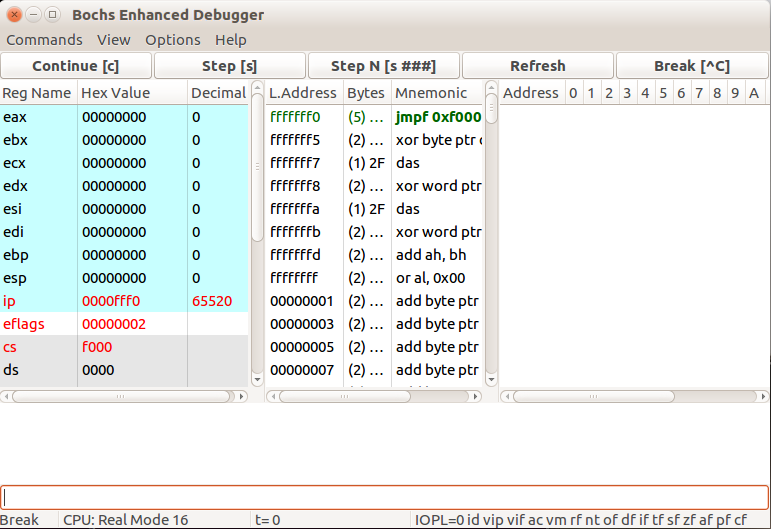
\includegraphics[scale=0.3]{img/bochs.png} & 	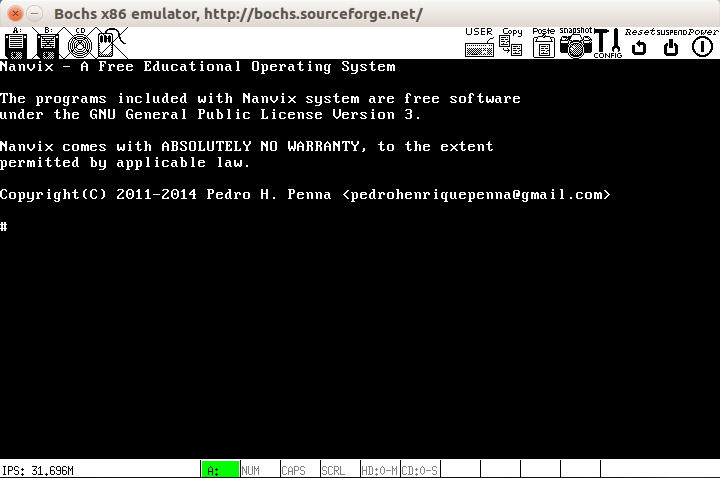
\includegraphics[scale=0.33]{img/nanvix.png} \\
	\end{tabular}
	\caption{(a) Bochs Debugger. (b) Nanvix.}
	\label{fig:bochs}
\end{figure}

\section{Nanvix em uma Máquina Virtual (VM)}
\label{sec:vm}

As seções anteriores mostraram como o Nanvix pode ser instalado e
utilizado em um sistema Linux com permissão de super-usuário. Porém, se
você utliza Windows (ou Linux sem permissão de super-usuário) será
necessário instalar e executar o Nanvix em uma Máquina Virtual (VM).
Nesse caso, aconselhamos a utilização do \textit{Virtual Box}
(disponível em \url{www.virtualbox.org}). No moodle da disciplina você encontrará uma VM para o \textit{Virtual Box} com um sistema operacional \textit{Lubuntu} instalado. Essa VM \textbf{já possui todas as ferramentas de desenvolvimento para o Nanvix instaladas}. Portanto, \textbf{não será necessário executar os procedimentos descritos na Seção~\ref{sec:ferramentas}} (você precisará somente executar os passos das Seções~\ref{sec:codigo} e~\ref{sec:compilacao}).

A senha do usuário desse sistema é ``\textbf{user}''.

\end{document}
